\subsection{Скорости $\beta^-$-распадов} \label{sec:weakfit}
  Помимо реакций нейтронного захвата, важную роль в $r$-процессе играют $\beta^-$-распады, которые увеличивают зарядовое число распадающегося ядра и тем самым обеспечивают естественный синтез новых химических элементов. При моделировании $r$-процесса важно убедиться, что для каждого ядра в нейтроноизбыточной области, нарабатывающегося в результате реакций $(n,\gamma)$, имеются данные о слабом распаде.

Значения астрофизических скоростей слабых распадов экзотических ядер, как и в случае с реакцией нейтронного захвата, приходится искать при помощи теоретических моделей. Ряд расчетов скоростей $\beta$-распадов выполнен специально для применения в астрофизических приложениях и, в частности, для расчета $r$-процесса (см., например, работы~\cite{moller2003, panov2016}). Большой массив скоростей слабых распадов, рассчитанных при помощи модели FRDM+QRPA~\cite{moller2003}, содержится в базе данных астрофизических скоростей реакций REACLIB~\cite{reaclib2010}.

\subsubsection{Зависимость скорости $\beta$-распада от массы ядра}
  Очевидно, что скорость $\beta$-распада должна сильно зависеть от массы исходного ядра. На это указывает хорошо известное правило Сарджента $\lambda \sim Q_\beta^5$, связывающее скорость распада $\lambda$ с энерговыделением $Q_\beta$, которое зависит от энергий связи начального и конечного ядер. Экспериментальные данные, позволяющие говорить о степенной связи скорости $\beta$-распада $\lambda$ с $Q_\beta$, были представлены Сарджентом в~\cite{sargent1933}. Таким образом вариации теоретической массовой модели должны влиять на результаты моделирования $r$-процесса не только через реакции $(n,\gamma)$, но и через слабые распады. 

  В условиях астрофизического $r$-процесса по его определению характерные времена $\beta^-$-распадов превышают скорости реакции $(n,\gamma)$ на порядки. Таким образом при моделировании $r$-процесса, в особенности на коротких промежутках времени порядка $1$~с, можно ожидать, что влияние неопределенностей теоретических значений скоростей слабых распадов будет незначительно в сравнении с неопределенностями расчета скоростей захвата нейтрона, обусловленных той же вариацией массовой модели. Исходя из этих соображений, в настоящей работе мы использовали скорости $\beta$-распадов из библиотеки REACLIB для всех трех наборов скоростей $(n,\gamma)$, полученных при помощи разных таблиц теоретических ядерных масс.

\subsubsection{Недостаток данных о скоростях $\beta^-$-распадов}
  После проведения расчета скоростей реакций нейтронного захвата на ядрах, входящих в используемые в настоящей работе таблицы теоретических масс, оказалось, что в REACLIB отсутствуют скорости слабых распадов для некоторых ядер-продуктов.  Это было ожидаемо, ведь разные ядерные модели по-разному предсказывают не только энергии связи, но и границы области существования ядер, определяемые знаком энергий отделения протона $B_p$ и нейтрона $B_n$ (см. формулы~\ref{eq:driplines}). Кроме того, как отмечалось ранее, в теоретических таблицах массы изотопов даны с некоторым запасом в область за границей существования ядер, и объем этого запаса разнится от таблицы к таблице. 

  На рис.~\ref{img:weak_comparison} синим цветом отмечены ядра, слабые распады которых внесены в библиотеку REACLIB, а оранжевым --- ядра из таблицы HFB-24, для которых в REACLIB отсутствуют данные по слабым распадам. Если добавить такие реакции $(n,\gamma)$ в REACLIB без соответствующих распадов, то их продукты будут накапливаться, приводя к некорректным результатам моделирования $r$-процесса. Похожую картину можно видеть для таблицы LMR2021. Для таблицы FRDM2012 область недостатка данных о $\beta$-распадах минимальна, так как модель слабых распадов, используемая в REACLIB, основана на массовой модели FRDM2012.
  

\begin{figure}
  \centering
  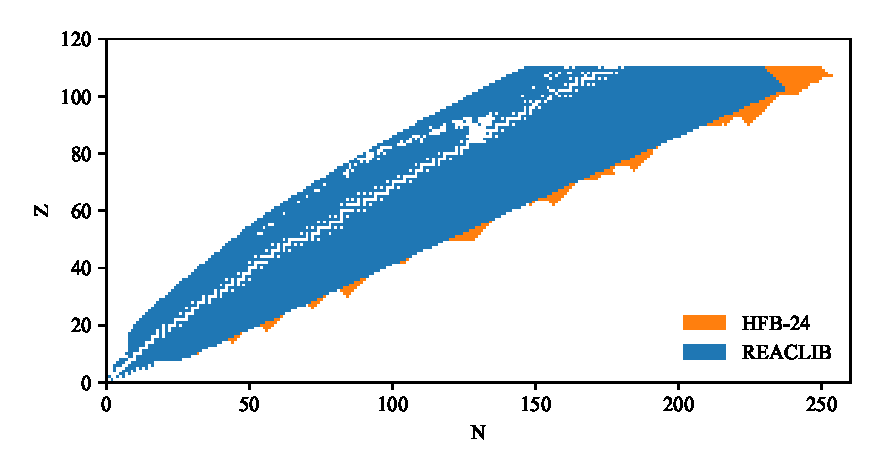
\includegraphics[width=0.8\textwidth]{pics/chart_weak_comparison.eps}
  \caption{Данные о слабых распадах из библиотеки REACLIB (синие квадраты) и нейтроноизбыточные изотопы, присутствующие в таблице масс HFB-24, но отсутствующие в REACLIB (оранжевые квадраты).}
  \label{img:weak_comparison}
\end{figure}

  Как было отмечено выше, скорости $\beta^-$-распадов в $r$-процессе существенно ниже скоростей $(n,\gamma)$ и влияние масс ядер на периоды полураспада не должно заметно сказываться на результатах моделирования $r$-процесса. В связи с этим мы решили ограничиться простой экстраполяцией в область нейтронного избытка для определения недостающих скоростей слабых распадов, используя в качестве исходных данных присутствующие в библиотеке REACLIB скорости. 

\subsubsection{Слабые распады с вылетом нейтронов}
  В библиотеке REACLIB для изотопов с избытком нейтронов помимо обычных $\beta^-$-распадами присутствуют $\beta^-$-распады с вылетом $1-3$ нейтронов. На рис.~\ref{img:decays_tb} показаны скорости слабых распадов нейтроноизбыточных изотопов тербия. Как видно, начиная с изотопа Tb$^{175}$ над $\beta^-$-распадом начинает преобладать распад $\text{Tb}^A \rightarrow \text{Dy}^{A-1} + \text{n}$, а с углублением в область нейтронного избытка усиливаются каналы с вылетом 2 и 3 нейтронов. Более того, начиная с $A = 185$ скорости $\beta^-$-распада падают до пренебрежимо малых значений. При этом видно, что сумма скоростей всех четырех каналов распада для каждого изотопа в зависимости от массового числа может быть аппроксимирована простой функцией, например, полиномом второй степени.

  Суммирование скорости $\beta^-$-распадов с вылетом разного числа нейтронов с точки зрения задачи расчета $r$-процесса имеет смысл, даже несмотря на то, что продукты этих распадов различаются числом нейтронов. При скоростях реакции $(n,\gamma)$, на порядки превосходящих скорости $\beta^-$-распадов, небольшие различия в числе нейтронов между изотопами одного химического элемента перестают играть большую роль, так продукт распада сразу же начнет интенсивного поглощать нейтроны. Причем предел, до которого ядро в $r$-процессе может насыщаться нейтронами, определяется не столько слабыми распадами, сколько статистическим равновесием между реакцией нейтронного захвата $(n,\gamma)$ и обратной реакцией фотовыбивания нейтрона $(\gamma,n)$. Это позволило нам при добавлении отсутствующих скоростей слабых распадов в REACLIB ограничиться только $\beta^-$-распадами. Такое допущение обусловлено спецификой $r$-процесса и может быть неприменимо для моделирования других процессов астрофизического нуклеосинтеза. 

\begin{figure}
  \centering
  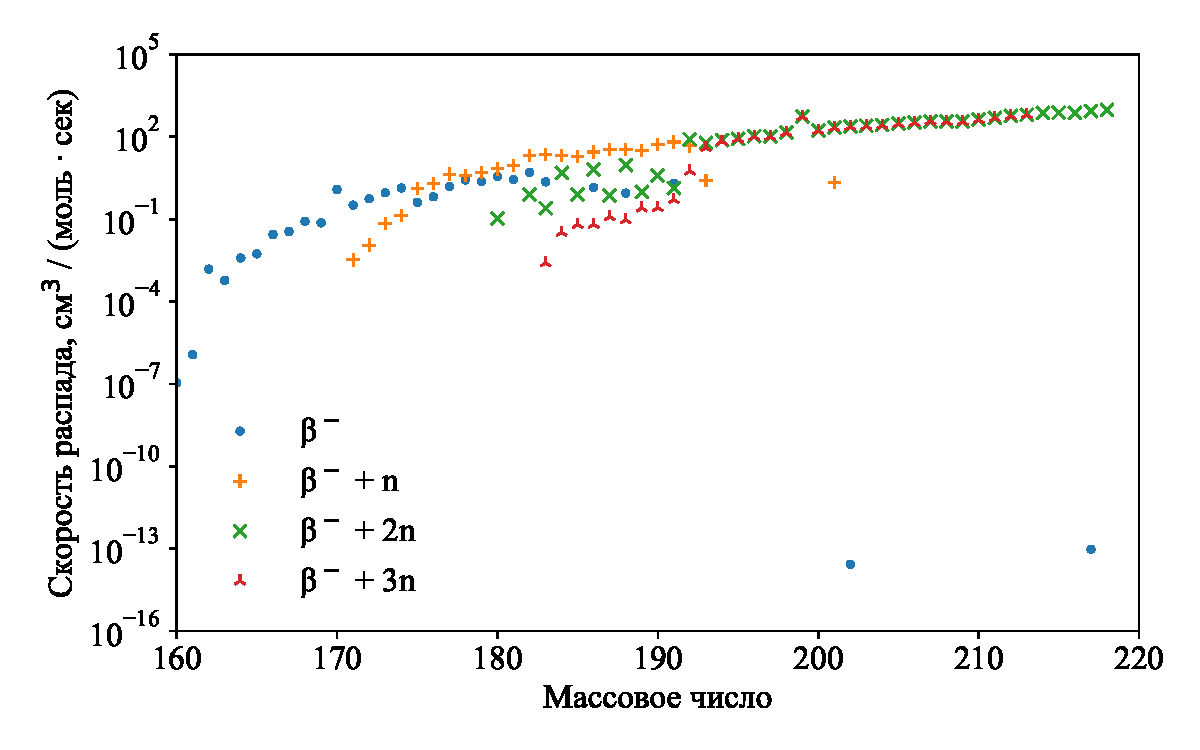
\includegraphics[width=0.7\textwidth]{pics/decays_tb.pdf}
  \caption{Скорости слабых распадов нейтроноизбыточных изотопов тербия, содержащиеся в библиотеке REACLIB. Различными маркерами отмечены $\beta^-$-распады с вылетом разного числа нейтронов. Скорости ниже $10^{-16}$~$\frac{\text{см}^3}{\text{моль}\cdot\text{сек}}$ не показаны.}
  \label{img:decays_tb}
\end{figure}

\subsubsection{Аппроксимация скоростей слабых распадов}
  Выборки исходных данных для аппроксимаций составлялись из сумм скоростей слабых распадов, независимо от числа вылетающих нейтронов, для каждого нейтроноизбыточного изотопа заданного химического элемента. Критерий нейтроноизбыточности, который мы используем в настоящей работе, описан в разделе~\ref{sec:nrich_criteria}.
  
  В качестве простейшей модельной функции для экстраполяции зависимости скоростей слабых распадов от массового числа может быть использован полином второй степени. Эта функция не отражает физики процесса, однако имеет всего три параметра аппроксимации и не требует большого числа исходных точек. 

  Более качественную модельную функцию можно получить, используя правило Сарджента $\lambda \sim Q_\beta^5$. Энерговыделение $Q_\beta$ может быть связано с массовым числом $A$ через формулу Вайцзеккера для энергии связи. Тогда зависимость скорости распада $\lambda$ от массового числа $A$ при фиксированном зарядовом числе $Z$ может быть представлена в виде
\begin{equation}
\begin{gathered}
  \displaystyle
  \lambda = b_1 \cdot (Q_\beta(A) - b_2)^5,\\
  Q_\beta(A) = 
  a_1 - \frac{a_2}{A^{1/3}} - \frac{a_3}{A} + \frac{a_4}{A^{3/4}} \xi,
  \quad \xi =
  \begin{cases}
    +1& \quad\text{для четных} \\
    \hspace{11pt}0& \quad\text{для нечетных} \\
    -1& \quad\text{для нечетно-нечетных}
  \end{cases},
\end{gathered}
\end{equation}
где $a_1$, $a_2$, $a_3$, $a_4$, $b_1$, $b_2$ --- параметры аппроксимации. Чтобы снизить число параметров, можно опустить член формулы Вайцзеккера, отвечающий за чётность (параметр $a_4$), не слишком сильно потеряв в точности.

  На рис.~\ref{fig:decay_fit} показаны примеры аппроксимаций скоростей слабых распадов нейтроноизбыточных изотопов тербия и свинца из библиотеки REACLIB, выполненных с использованием описанных модельных функций. Как видно, различия между двумя экстраполяциями несущественны, хотя экстраполированные значения, полученные с помощью правила Сарджента, обычно превосходят параболическую экстраполяцию в области сильного нейтронного избытка.
  
  В настоящей работе мы использовали аппроксимацию по правилу Сарджента для большинства ядер, а к параболической модельной функции прибегали лишь в случае недостаточных размеров массива исходных данных.
  
\begin{figure}
  \centering
  \begin{subfigure}{0.48\textwidth}
    \centering
    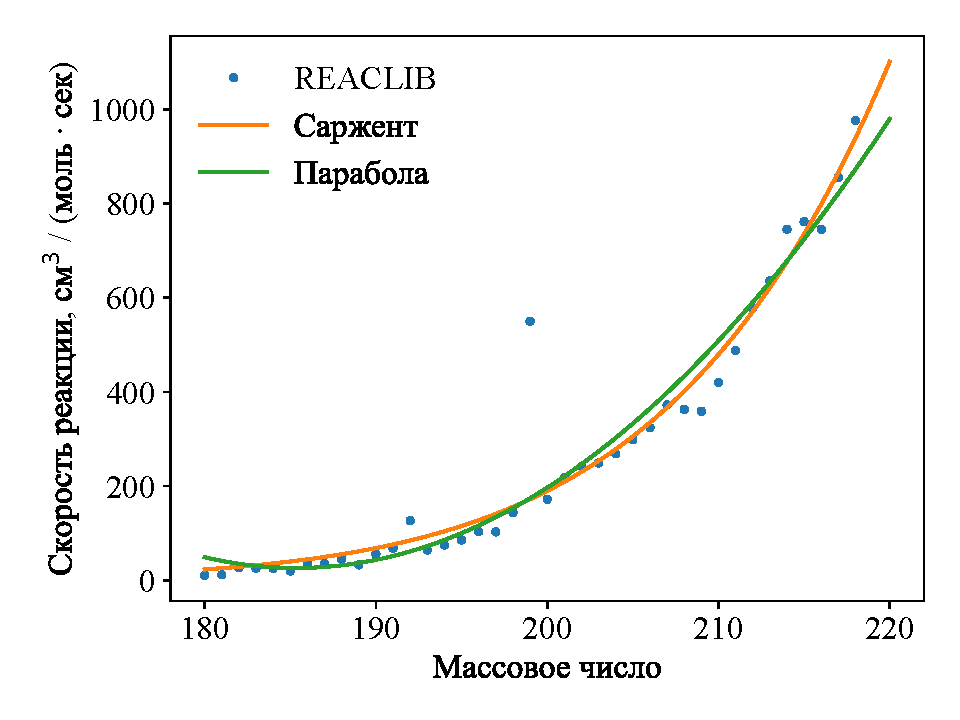
\includegraphics[width=\textwidth]{pics/decay_fit65.pdf}
    \caption{Тербий}
  \end{subfigure}
  \hfill
  \begin{subfigure}{0.48\textwidth}
    \centering
    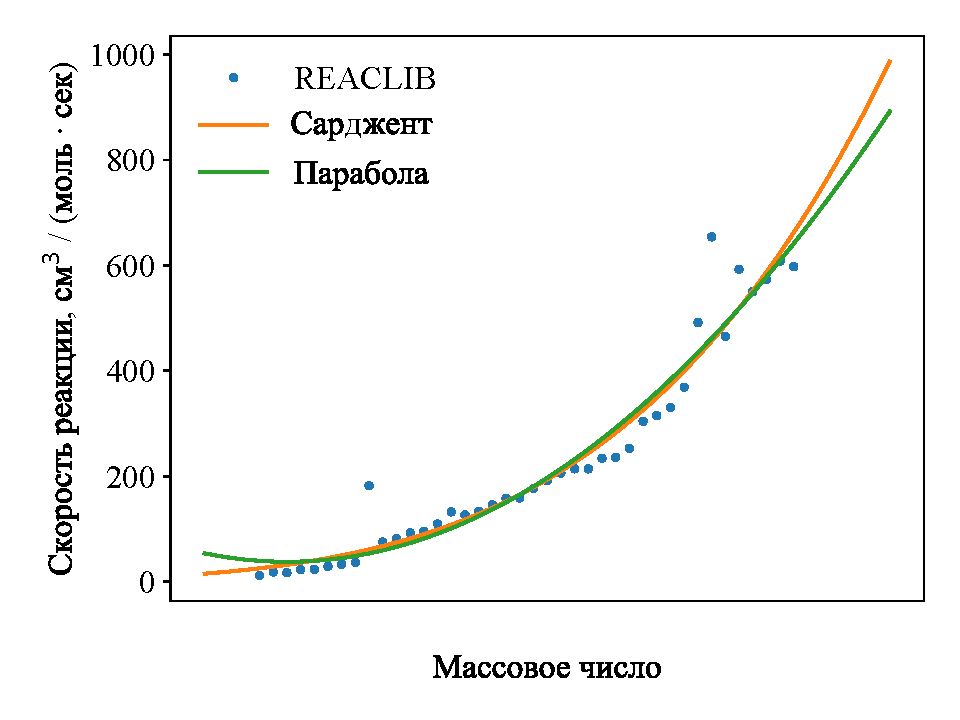
\includegraphics[width=\textwidth]{pics/decay_fit82.pdf}
    \caption{Свинец}
  \end{subfigure}
  \caption{Экстраполяция скоростей слабых распадов для нейтроноизбыточных ядер на основе данных из библиотеки REACLIB двумя модельными функциями: полиномом второй степени и формулой скорости $\beta$-распада на основе правила Сарджента и формулы Вайцзеккера.}
  \label{fig:decay_fit}
\end{figure}

\subsubsection{Особенность слабых распадов из библиотеки REACLIB}
  Отметим, что в библиотеке REACLIB все слабые распады имеют постоянные значения, не зависящие от температуры. При этом ясно, что в зависимости от температуры среды меняется заселенность энергетических уровней ядра, от которой зависят скорости $\beta$-распадов. В описании базы данных~\cite{reaclib2010} упоминается, что, хотя учет возбужденных состояний может существенно повлиять на периоды полураспадов, в текущей версии REACLIB в библиотеку включены экспериментальные и теоретические скорости $\beta$-распадов лишь в земных условиях, однако они могут быть замещены в дальнейшем астрофизическими скоростями, завясящими от температур и плотностей среды.
